% -*- coding: utf-8; -*-

\chapter{Introdução}
\label{intro}
	Visualização volumétrica é a vertente da computação gráfica caracterizada por visualizar campos escalares, isto é, representar visualmente um volume de dados que relaciona um valor escalar a um ponto no espaço. Esses dados podem vir de inúmeras fontes, desde exames médicos de ressonância magnética (RM) e tomografia computadorizada (TC) a simulações físicas, como em reservatórios de petróleo e fraturas em materiais. Um campo escalar também pode ser interpretado como a variação de uma determinada informação num espaço delimitado. Por exemplo, um exame de tomografia computadorizada informa como a densidade da estrutura fisiológica varia naquela região em que foi escaneada, como visto na figura~\ref{fig:head_ct_slice_intro}, onde a cor preta indica a menor densidade e a cor branca a maior.
    
    Um componente essencial da visualização volumétrica é a função de transferência (FT): um mapeamento feito entre voxels do volume renderizado e um ou mais atributos que compõem suas propriedades ópticas, como por exemplo, cor e opacidade. Ou seja, através da função de transferência é possível definir como cada elemento do volume de dados será visto na imagem final. Um objetivo prático do uso de FTs seria, dado uma TC da cabeça de um indivíduo, visualizar apenas seu crânio. Essa prática auxilia os médicos no exame e diagnóstico de pacientes, o que mostra o quanto pode ser importante utilizar funções de transferência. As imagens na figura~\ref{fig:head_skull_intro} mostram visualizações volumétricas da tomografia apresentada na figura~\ref{fig:head_ct_slice_intro}, utilizando diferentes funções de transferência.

\begin{figure}[h]
	\centering
	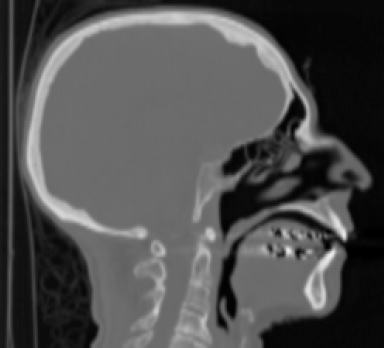
\includegraphics[width=0.3\textwidth]{images/head_ct_slice_intro}
    \caption{Fatia da tomografia computadorizada da cabeça de um indivíduo~\cite{gordonms}.}
    \label{fig:head_ct_slice_intro}
\end{figure}
\begin{figure}[h]
	\centering
    \subfigure[]{
    	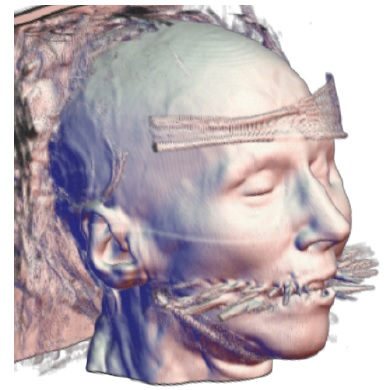
\includegraphics[width=0.3\textwidth]{images/head_ct_intro}
    }
    \subfigure[]{
    	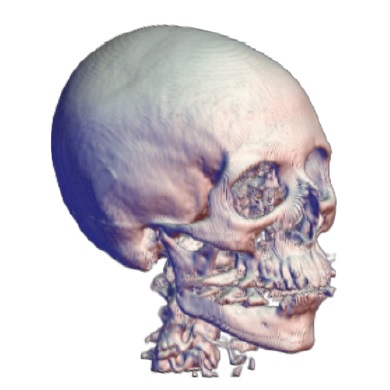
\includegraphics[width=0.3\textwidth]{images/head_skull_intro}
    }
    \caption{Visualização volumétrica da mesma TC apresentada na figura~\ref{fig:head_ct_slice_intro} a partir de diferentes funções de transferência~\cite{gordonms}.}
    \label{fig:head_skull_intro}
\end{figure}
    
    No entanto, obter FTs que isolem corretamente estruturas internas do volume, ou que simplesmente resultem em uma visualização adequada de toda a estrutura de interesse, não é uma tarefa fácil para um usuário comum. Definir manualmente uma função de transferência é um trabalho repetitivo de tentativa e erro, que exige paciência e um conhecimento mínimo sobre os dados sendo visualizados. Por esse motivo, a busca por métodos automáticos é tão importante e vem sendo desenvolvida há mais de 20 anos.
    
    Em 1998, \textit{Kindlmann e Durkin}~\cite{gordon} promoveram um grande salto no estado da arte com seu método semiautomático. Alguns trabalhos que vieram a seguir buscaram o mesmo objetivo: automatizar a criação de FTs que destacassem as fronteiras entre diferentes materiais do volume, permitindo ao usuário um controle fino sobre a função obtida. Mas a maioria das pesquisas que se sucederam resultaram em um aprimoramento da interface com o usuário. Através de histogramas 2D, regiões de possíveis fronteiras são reveladas, cabendo então ao usuário selecioná-las, atribuindo cor e opacidade.
    
    Esse tipo de abordagem dá ao usuário controle total sobre a função de transferência que será gerada, ao mesmo tempo que as interfaces sofisticadas minimizam a necessidade de se conhecer os dados sendo visualizados. Contudo, esses trabalhos retomam o processo repetitivo de tentativa e erro. Além disso, como a relação entre as regiões dos histogramas e os materiais do volume não são intuitivas, a interface apresenta um novo desafio ao usuário.
    
    Durante esses anos, a grande maioria das pesquisas têm analisado seus resultados na área médica, sem avaliar a aplicabilidade de tais métodos em outros dados científicos. Como consequência, os métodos desenvolvidos exploram apenas malhas estruturadas, deixando de lado dados representados por malhas não estruturadas, como reservatórios de petróleo, por exemplo.
    
    Segundo \textit{Rosa et al. 2006, p. xii, p. 517}~\cite{rosa}, um dos métodos mais sofisticados para se estimar características e prever o comportamento de reservatórios de petróleo é utilizar simulação numérica. A simulação permite, por exemplo, determinar as melhores condições para a produção de petróleo, assim como estimar o volume de óleo e gás que poderá ser extraído durante a exploração do reservatório.
    
    Assim como no caso dos volumes médicos, a aplicação de FTs pode destacar regiões do reservatório, ou realçar a interface entre elas. Por exemplo, a área de contato entre a água e o óleo (denominada frente de avanço) é uma informação importante sobre o fluxo do reservatório. As frentes de avanço delimitam regiões importantes na fase de recuperação secundária de um reservatório e podem ser calculadas analiticamente, mas não visualizadas sem uma função de transferência apropriada.
    
\begin{figure}[h]
	\centering
    \subfigure[Simulação da saturação de óleo em um reservatório.]{
    	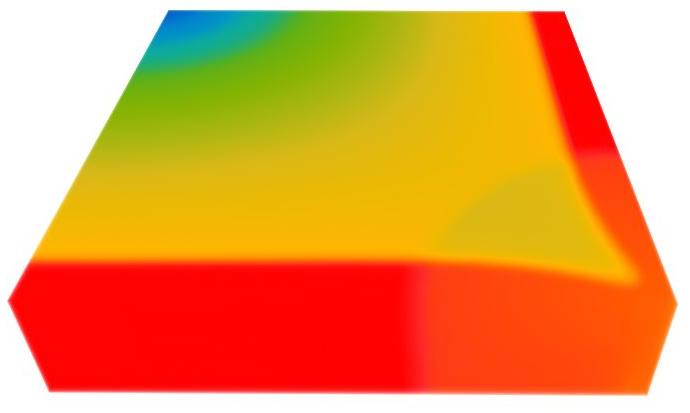
\includegraphics[width=0.4\textwidth]{images/reserv_intro}%
        \label{fig:reserv_intro}%
    }
    \subfigure[Realce da fronteira mais evidente da imagem ao lado.]{
    	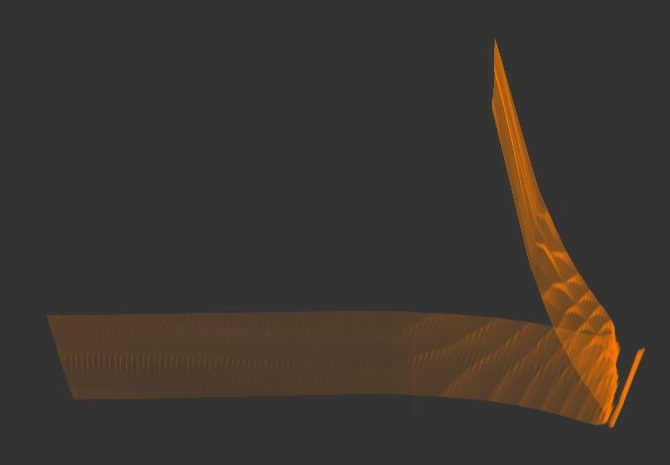
\includegraphics[width=0.4\textwidth]{images/reserv_tf_intro}%
        \label{fig:reserv_tf_intro}%
    }
    \caption{Visualização volumétrica de reservatório de petróleo.}
\end{figure}
    
    Com base na abordagem feita por \textit{Kindlmann e Durkin}~\cite{gordon} este trabalho desenvolve um novo método para geração automática de funções de transferência, com o objetivo de realçar fronteiras de um volume de dados. A técnica é voltada para malhas estruturadas e não estruturadas. Desta forma, são apresentados resultados para volumes sintéticos, volumes médicos e volumes de reservatório.

    No capítulo \ref{related} alguns trabalhos relacionados a este são comentados, realçando suas contribuições e questões em aberto que deram espaço a outros trabalhos. No capítulo \ref{gordon}, o método criado por \textit{Kindlmann e Durkin}~\cite{gordon} é explicado e avaliado segundo os objetivos e motivações deste trabalho. A abordagem proposta por essa dissertação é apresentada no capítulo \ref{my} e seus resultados e comparações avaliados no capítulo \ref{result}. Por fim, conclusões e trabalhos futuros são discutidos no capítulo \ref{conclusion}.